\scanpage{8}
Orientation of a contour.

Choice for every edge $a\in A$ of an ``orientation of $a$'' i.e. of an origin $\deleted{\unsure{o|\omega}}\sigma(a)$ of $a$, in such a way that we have

% slanted
\margin{\diagram{\begin{tikzcd}[ampersand replacement=\&,column sep=small] A \arrow[r,"{\substack{\sigma\\[-.35ex]\sim}}"] \& S \end{tikzcd}}
$\forall a\in A,\ \deleted{\unsure{\exists1|\exists}}(\sigma(a),a)\in R$\\
\deleted{$\unsure{\forall s\in S|\forall a\in S},\exists1\,a\in A,$}}

\[
\begin{aligned}
&\text{If}\quad \deleted{R\{s\}=\{a,b\},\ \text{then }\exists}\quad s\in S,\quad \exists1\ a\in R\{s\}\ \text{such that}\\
&s=\sigma(a).
\end{aligned}\tag*{(\unsure{O|0})}
\]

Reduction to the connected case

\uline{Proposition} If $(S,A,R)$ is a connected contour, it has exactly \uline{two} orientations ($\omega$ and $-\omega$).

\figure{
\begin{tikzpicture}[x=.02cm,y=.02cm]
\draw[->,line width=.6pt] (0,0) .. controls (18,-2) and (39,-2) .. (56,-1);
\fill (61,0) circle[radius=1.7];
\draw[->,line width=.65pt] (62,0) .. controls (75,5) and (92,15) .. (108,25);
\end{tikzpicture}}

\figure{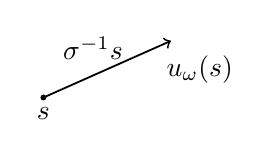
\begin{tikzpicture}[x=.03cm,y=.03cm]
\fill (0,0) circle[radius=1.25];\draw[->,line width=.65pt] (0,0)--(54,24);
\node[below] at (0,0) {$s$};
\node[above] at (21,12) {$\sigma^{-1}s$};
\node[below right] at (48,22) {$u_{\omega}(s)$};
\end{tikzpicture}}
\deleted{Proposition} \uline{Proposition} Let $\omega$ be an orientation of the contour $(S,A,R)$.

$\forall s\in S$, let $\deleted{\unsure{\omega(s)|w(s)}\unsure{u_{\omega}|u}}\inserted{u_{\omega}}(s)$ be the \uline{endpoint} of the unique edge \inserted{$\sigma^{-1}(s)$} which has \deleted{\unsure{as}} $s$ as origin
\[
\left[\begin{aligned}(u_{\omega}(s),\sigma^{-1}(s))&\in R,\\u_{\omega}(s)&\ne s\end{aligned}\right]
\]

\figure{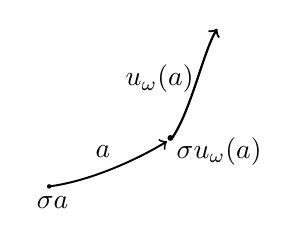
\begin{tikzpicture}[x=.022cm,y=.022cm]
\fill (0,0) circle[radius=1.3];\draw[->,line width=.7pt] (0,0) .. controls (23,3) and (50,15) .. (68,26);
\fill (70,28) circle[radius=1.7];\draw[->,line width=.8pt] (71,28) .. controls (82,44) and (89,78) .. (97,91);
\node[below] at (2,0) {$\sigma a$};\node[above] at (31,11) {$a$};
\node[right] at (68,20) {$\sigma u_{\omega}(a)$};\node[left] at (89,62) {$u_{\omega}(a)$};
\end{tikzpicture}}
$\forall a\in A$, let $u_{\omega}(a)$ be the unique arc of $S$ whose origin is the endpoint of $a$
\[
\left[\begin{aligned}
(\sigma u_{\omega}(a),a)&\in R,\quad \sigma u_{\omega}(a)\ne\sigma a\\
&\hspace{6em}\text{i.e.}\quad u_{\omega}(a)\ne a
\end{aligned}\right]
\]

\margin{$\big\}$}Then $u_{\omega}:(S,\deleted{\unsure{R|B}}A)\unsure{-|\to}(S,A)$ is an automorphism of the graph $(S,A,R)$. We have $u_{-\omega}=u_{\omega}^{-1}$. The automorphisms $u_{\omega},u_{\omega}^{-1}$ are characterized by the \deleted{fact that} equivalent conditions

$1^{\circ})$ $\forall s\in S$, $s$ linked to $gs$

$2^{\circ})$ $\forall a\in A$, $a$ linked to $ga$

If $n=\operatorname{card}S=\operatorname{card}A$, the order of $u_{\omega},u_{\omega}^{-1}=u_{-\omega}$ is $n$

\unsure{arrow|and} $u_{\omega}\ne u_{-\omega}$ if and only if $n\ne2$ i.e. $n\geq3$ ; therefore $\omega\longmapsto u_{\omega}$ is a bijection of $\operatorname{or}(S,A,R)$ with the set of $g\in\operatorname{Aut}(S,A,R)$ satisfying the equivalent conditions \unsure{$1^{\circ}$ or $2^{\circ}\big\}$|$1^{\circ}$ or $2^{\circ})\big\}$}, And the cyclic \unsure{group|group} $\simeq\mathbb{Z}/n\mathbb{Z}$ generated by $u_{\omega}$ is \deleted{\unsure{formed|form}} \inserted{the} \inserted{group $G^{\unsure{0|\circ}}$} of \inserted{oriented} automorphisms of $(S,A,R,\omega)$ \inserted{\unsure{read|the} of $S,A,R;\omega)$}. $S$ and $A$ are \uline{torsors} under $G^{0}$.

\deleted{\unsure{To give a|The datum of a}}

Torsor under $\mathbb{Z}/n\mathbb{Z}$ \inserted{$(n\geq1)$} $=$ set \deleted{\unsure{where}} with $n$ element equipped with a circular order $^{\times}$. To give a contour
% archive sheet number: 7
